\chapter{Functions}

This section deals with functions.
Functions serve to package a set of instructions.
For example, in this chapter we will see functions that serve
to remove or add edges and vertices.
In the case of edge removal, the function
\mintinline{ts}{removeEdge} packages the instructions
necessary to remove an edge from the network.

Networks are often used to represent real world
phenomena that are constantly changingç thus,
it is important to be able to dynamically remove
edges and nodes from a network.
In the aforementioned example of a social network,
this could mean someone deleting their account.

The functions for removing edges and vertices remove said elements of the network.

\begin{minted}[bgcolor=bg]{ts}
removeEdge(args:
          { from: base_id; to: base_id; id?: base_id }) {
  if (args.id !== undefined) {
    this.removeMultigraphEdge(args.id);
    return;
  } else if (this.is_multigraph) {
    throw { message: ERROR.UNDEFINED_ID, id: args.id };
  }

  this.edges.forEach(({ vertices }, id) => {
    if (this.checkEdgeIsSame(vertices, args)) {
      this.edges.delete(id);
      return;
    }
  });
}
\end{minted}

The \mintinline{ts}{removeVertex()} function differs itself from
\mintinline{ts}{removeEdge()}.
When a vertex is removed, all of the edges associated with it also have to be removed.
Returning to the social network example, we can say that, when
a user removes their account, their relationships to the remaining
users are also removed.

\begin{minted}[bgcolor=bg]{ts}
removeVertex(id: base_id) {
  if (!this.vertices.has(id))
    throw { message: ERROR.INEXISTENT_VERTICE, vertex: id };

  this.vertices.delete(id);

  this.edges.forEach(({ vertices }, key) => {
    const { from, to } = vertices;
    if (from === id || to === id)
      this.edges.delete(key)
  });
}
\end{minted}

An advantage of using \mintinline{ts}{Maps}
to store the network's vertices and edges is that it is easier to get
them by ID.
The function \mintinline{ts}{hasVertex()} takes advantage of
a vertex ID to quickly find whether a network contains a
vertex with the specified ID.

\begin{minted}[bgcolor=bg]{ts}
hasVertex(id: base_id): boolean {
  return this.vertices.has(id);
}
\end{minted}

To get an edge between two vertices, \mintinline{ts}{Array.prototype.find()}
is used in the \mintinline{ts}{edge_list} array.
The \mintinline{ts}{find()}
function returns the first element in a list that fulfills the given property.
Here, we can see how the conversion from an edge map to a list of edges
can be useful.

The \mintinline{ts}{edgeBetween()} function will return the edge with the given nodes if it exists,
otherwise it is undefined.

\begin{minted}[bgcolor=bg]{ts}
/**
 * Returns the edge between two nodes.
 * @param  {base_id} from
 * @param  {base_id} to
 * @returns base_id[]
 */
edgeBetween(
  from: base_id,
  to: base_id,
  is_directed = this.is_directed
): Edge | undefined {
  return this.edge_list.find(({ vertices }) =>
    this.checkEdgeIsSame(vertices, { from, to }, is_directed)
  );
}
\end{minted}

To check if two edges are the same
(if they have the same \mintinline{ts}{from} and \mintinline{ts}{to} properties),
the private function \mintinline{ts}{checkEdgeIsSame()} is used.

A private function can only be accessed inside the class declaration,
and is not meant to be used outside of it.

The \mintinline{ts}{checkEdgeIsSame()} function will take in two edges and compare their nodes
(\mintinline{ts}{from} and \mintinline{ts}{to}).
If a network is directed, \mintinline{ts}{from} is compared with \mintinline{ts}{from},
and \mintinline{ts}{to} is compared with \mintinline{ts}{to}.
If it is undirected the comparison between \mintinline{ts}{to} and \mintinline{ts}{from}
also need to be performed.
Thus, the function also receives an \mintinline{ts}{is_directed} property.

\begin{minted}[bgcolor=bg]{ts}
checkEdgeIsSame(
  edge_a: EdgeArgs,
  edge_b: EdgeArgs,
  is_directed = this.is_directed
): boolean {
  if (edge_a.from === edge_b.from && edge_a.to === edge_b.to)
    return true;
  else if (
    edge_a.to === edge_b.from &&
    edge_a.from === edge_b.to &&
    !is_directed
  )
    return true;
  return false;
}
\end{minted}

The way an edge check works depends on whether or not a network is directed.
Nevertheless, it is also possible to force an undirected check.

A forced undirected check is useful when it is only necessary to know
if an edge between $A$ and $B$ exists at all, 
instead of whether a \textit{directed} edge from $A$ to $B$ exists.

There are two functions that serve mostly as a convenience.
They are ID functions which help create new IDs that can be assigned to new edges or vertices.
On the user level, there is seldom any reason to assign IDs to edges.
However, because the network uses \mintinline{ts}{Maps}, every edge needs to have
an ID assigned to it.
The \mintinline{ts}{newEID()} function generates a valid ID to be used internally.

\begin{minted}[bgcolor=bg]{ts}
  newVID(): base_id {
   let id = this.free_vid++;
   while (this.vertices.has(id)) {
     id = Math.floor(Math.random() * this.vertex_limit);
   }
   return id;
 }
 
 newEID() {
   let id = this.free_eid++;
   while (this.edges.has(id)) {
     id = Math.floor(Math.random() * this.edge_limit);
   }
   return id;
 }
\end{minted}

There are four special ways to add edges and vertices to a network.
These exist as a shorthand to add vertices and edges.
It is useful to be able to add multiple edges to a network at
the same time.

\begin{minted}[bgcolor=bg]{ts}
 addEdgeMap(edge_map: Map<base_id, Edge>) {
  edge_map.forEach((edge, id) => this.edges.set(id, edge));
}

addEdgeList(edge_list: EdgeArgs[]) {
  edge_list.forEach((edge_args, id) =>
    this.edges.set(id, new Edge(edge_args))
  );
}

 addVertexMap(vertex_map: Map<base_id, Vertex>) {
  vertex_map.forEach((vertex, id) =>
    this.vertices.set(id, vertex));
}

addVertexList(vertex_list: VertexArgs[]) {
  vertex_list.forEach((vertex_args, id) =>
    this.vertices.set(id, new Vertex(vertex_args))
  );
}
\end{minted}

An array of edges could be added as such:

\begin{minted}[bgcolor=bg]{ts}
const edge_list = [
  [2,3],
  ['b',3]
]

net.addEdgeList(edge_list)
\end{minted}

This abstracts the complexity of adding multiple edges at the same time
from the user.
The code above is much simpler and easier to understand than the
following example:

\begin{minted}[bgcolor=bg]{ts}
const edge_list = [
  [2,3],
  ['b',3]
]

edge_list.forEach(edge =>
    net.addEdge({from: edge[0], to: edge[1]})
);
\end{minted}

\begin{figure}[H]
  \centering
  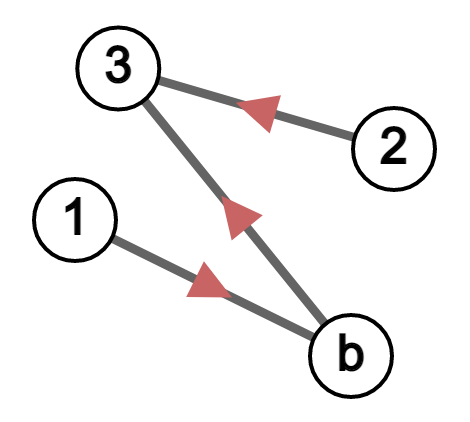
\includegraphics[scale=.25]{img/net_1b_edge_list.png}
  \caption{Our previous `net', now with the list of edges added.}
  \label{fig:net_edge_list}
\end{figure}

Other utility functions are:

\begin{minted}[bgcolor=bg]{ts}
hasEdge(from: base_id,
        to: base_id,
        is_directed = false): boolean {
  return this.edge_list.some(({ vertices }) =>
    this.checkEdgeIsSame(vertices, { from, to }, is_directed)
  );
}

getEdgesBetween(
  from: base_id,
  to: base_id,
  is_directed = this.is_directed
): base_id[] | base_id {
  let edge_list: base_id[] = [];

  this.edges.forEach(({ vertices }, id) => {
    if (this.checkEdgeIsSame(
                              vertices,
                              { from, to },
                              is_directed
                            )) {
      edge_list.push(id);
    }
  });

  return this.is_multigraph ? edge_list : edge_list[0];
}

addVertex(args: VertexArgs) {
  if (this.vertices.size >= this.vertex_limit)
    throw { message: ERROR.VERTICE_LIMIT };
  if (args.id !== undefined && this.vertices.has(args.id))
    throw { message: ERROR.EXISTING_VERTICE };

  this.vertices.set(args.id, new Vertex(args));
}
\end{minted}

The \mintinline{ts}{addEdge()} function looks different from the
\mintinline{ts}{addVertex()} function because it has to deal with many exceptions.

The main addition to \mintinline{ts}{addEdge()} is the \mintinline{ts}{do_force} argument.
It is set to true by default.
When \mintinline{ts}{addEdge()} is called,
it first checks if the vertices you are trying to connect exists.
If they don't and \mintinline{ts}{do_force=true},
the function will add the vertices to the network automatically.

\begin{minted}[bgcolor=bg]{ts}
addEdge(args: EdgeArgs) {
  args.do_force ??= true;
  args.weight ??= 1;
  args.id ??= this.newEID();
  if (this.edges.has(args.id))
    throw { message: ERROR.EXISTING_EDGE };
  if (this.edges.size >= this.edge_limit)
    throw { message: ERROR.EDGE_LIMIT };
  if (!args.do_force) {
    if (!this.vertices.has(args.from))
      throw {
        message: ERROR.INEXISTENT_VERTICE,
        vertex: args.from
      };
    if (!this.vertices.has(args.to))
      throw {
        message: ERROR.INEXISTENT_VERTICE,
        vertex: args.to
      };
  } else {
    if (!this.vertices.has(args.from))
      this.addVertex({ id: args.from });
    if (!this.vertices.has(args.to))
      this.addVertex({ id: args.to });
  }
  if (!this.is_multigraph &&
      this.hasEdge(args.from, args.to))
    return;
  this.edges.set(args.id, new Edge(args));
}
\end{minted}

In the following code, vertices `1' and `2' are created by \mintinline{ts}{addEdge()}
before it adds an edge to net.

\begin{minted}[bgcolor=bg]{ts}
const net = new Network()
net.addEdge({ from: 1, to: 2 })
\end{minted}

If the edge should only be added if the network already has the given vertices,
\mintinline{ts}{do_force} can be set to false:

\begin{minted}[bgcolor=bg]{ts}
const net = new Network()
net.addEdge({ from: 1, to: 2, do_force: false })
\end{minted}

The previous code will throw an error, since \mintinline{ts}{addEdge()}
will not try to force the creation of the edge by
adding vertices `1' and `2' to net.

There are also some private utility functions used in algorithms
that will be explained in the next chapter.

\begin{minted}[bgcolor=bg]{ts}
listHasTriplet(triplet_arr: Triplet[],
                triplet: Triplet): boolean {
  return !!triplet_arr.find((trip) =>
    this.isSameTriplet(triplet, trip));
}

isSameTriplet(arr1: Triplet, arr2: Triplet): boolean {
  if (arr1.length !== arr2.length) return false;
  return arr1.every((element, index) =>
    element === arr2[index]);
}
\end{minted}
